\section{新仓规则: 方案研究}
\subsection{POC: JAR定义接口、吊挂实现接口}
\begin{enumerate}
	\item \bf{JAR定义接口}
	\begin{lstlisting}
package ncdc.jar;

import java.util.List;

public interface IDataFromHangerApp {
    /**
     * Proof of concept: 验证JAR包定义接口，吊挂App实现接口
     * @return List<String>: 库区名称列表
     */
    List<String> getStockAreaList();
}
	\end{lstlisting}\vspace{-30pt}
	
	\item \bf{APP（吊挂）实现接口}
	\begin{lstlisting}
package ncdc.app.interface2jar;

import ncdc.jar.IDataFromHangerApp;
import java.util.Arrays;
import java.util.List;

public class IDataFromHangerAppImpl implements IDataFromHangerApp {
    static IDataFromHangerAppImpl instance = null;
    @Override
    public List<String> getStockAreaList() {
        return Arrays.asList("A","B","C");
    }

    public static IDataFromHangerAppImpl getInstance() {
        if (instance == null) {
            instance = new IDataFromHangerAppImpl();
        }
        return instance;
    }

    private IDataFromHangerAppImpl() {}
}
	\end{lstlisting}\vspace{-30pt}
	
	\item \bf{APP将接口实现类对象传递给JAR}
	\begin{figure}[H]%[htbp!]
		\centering
		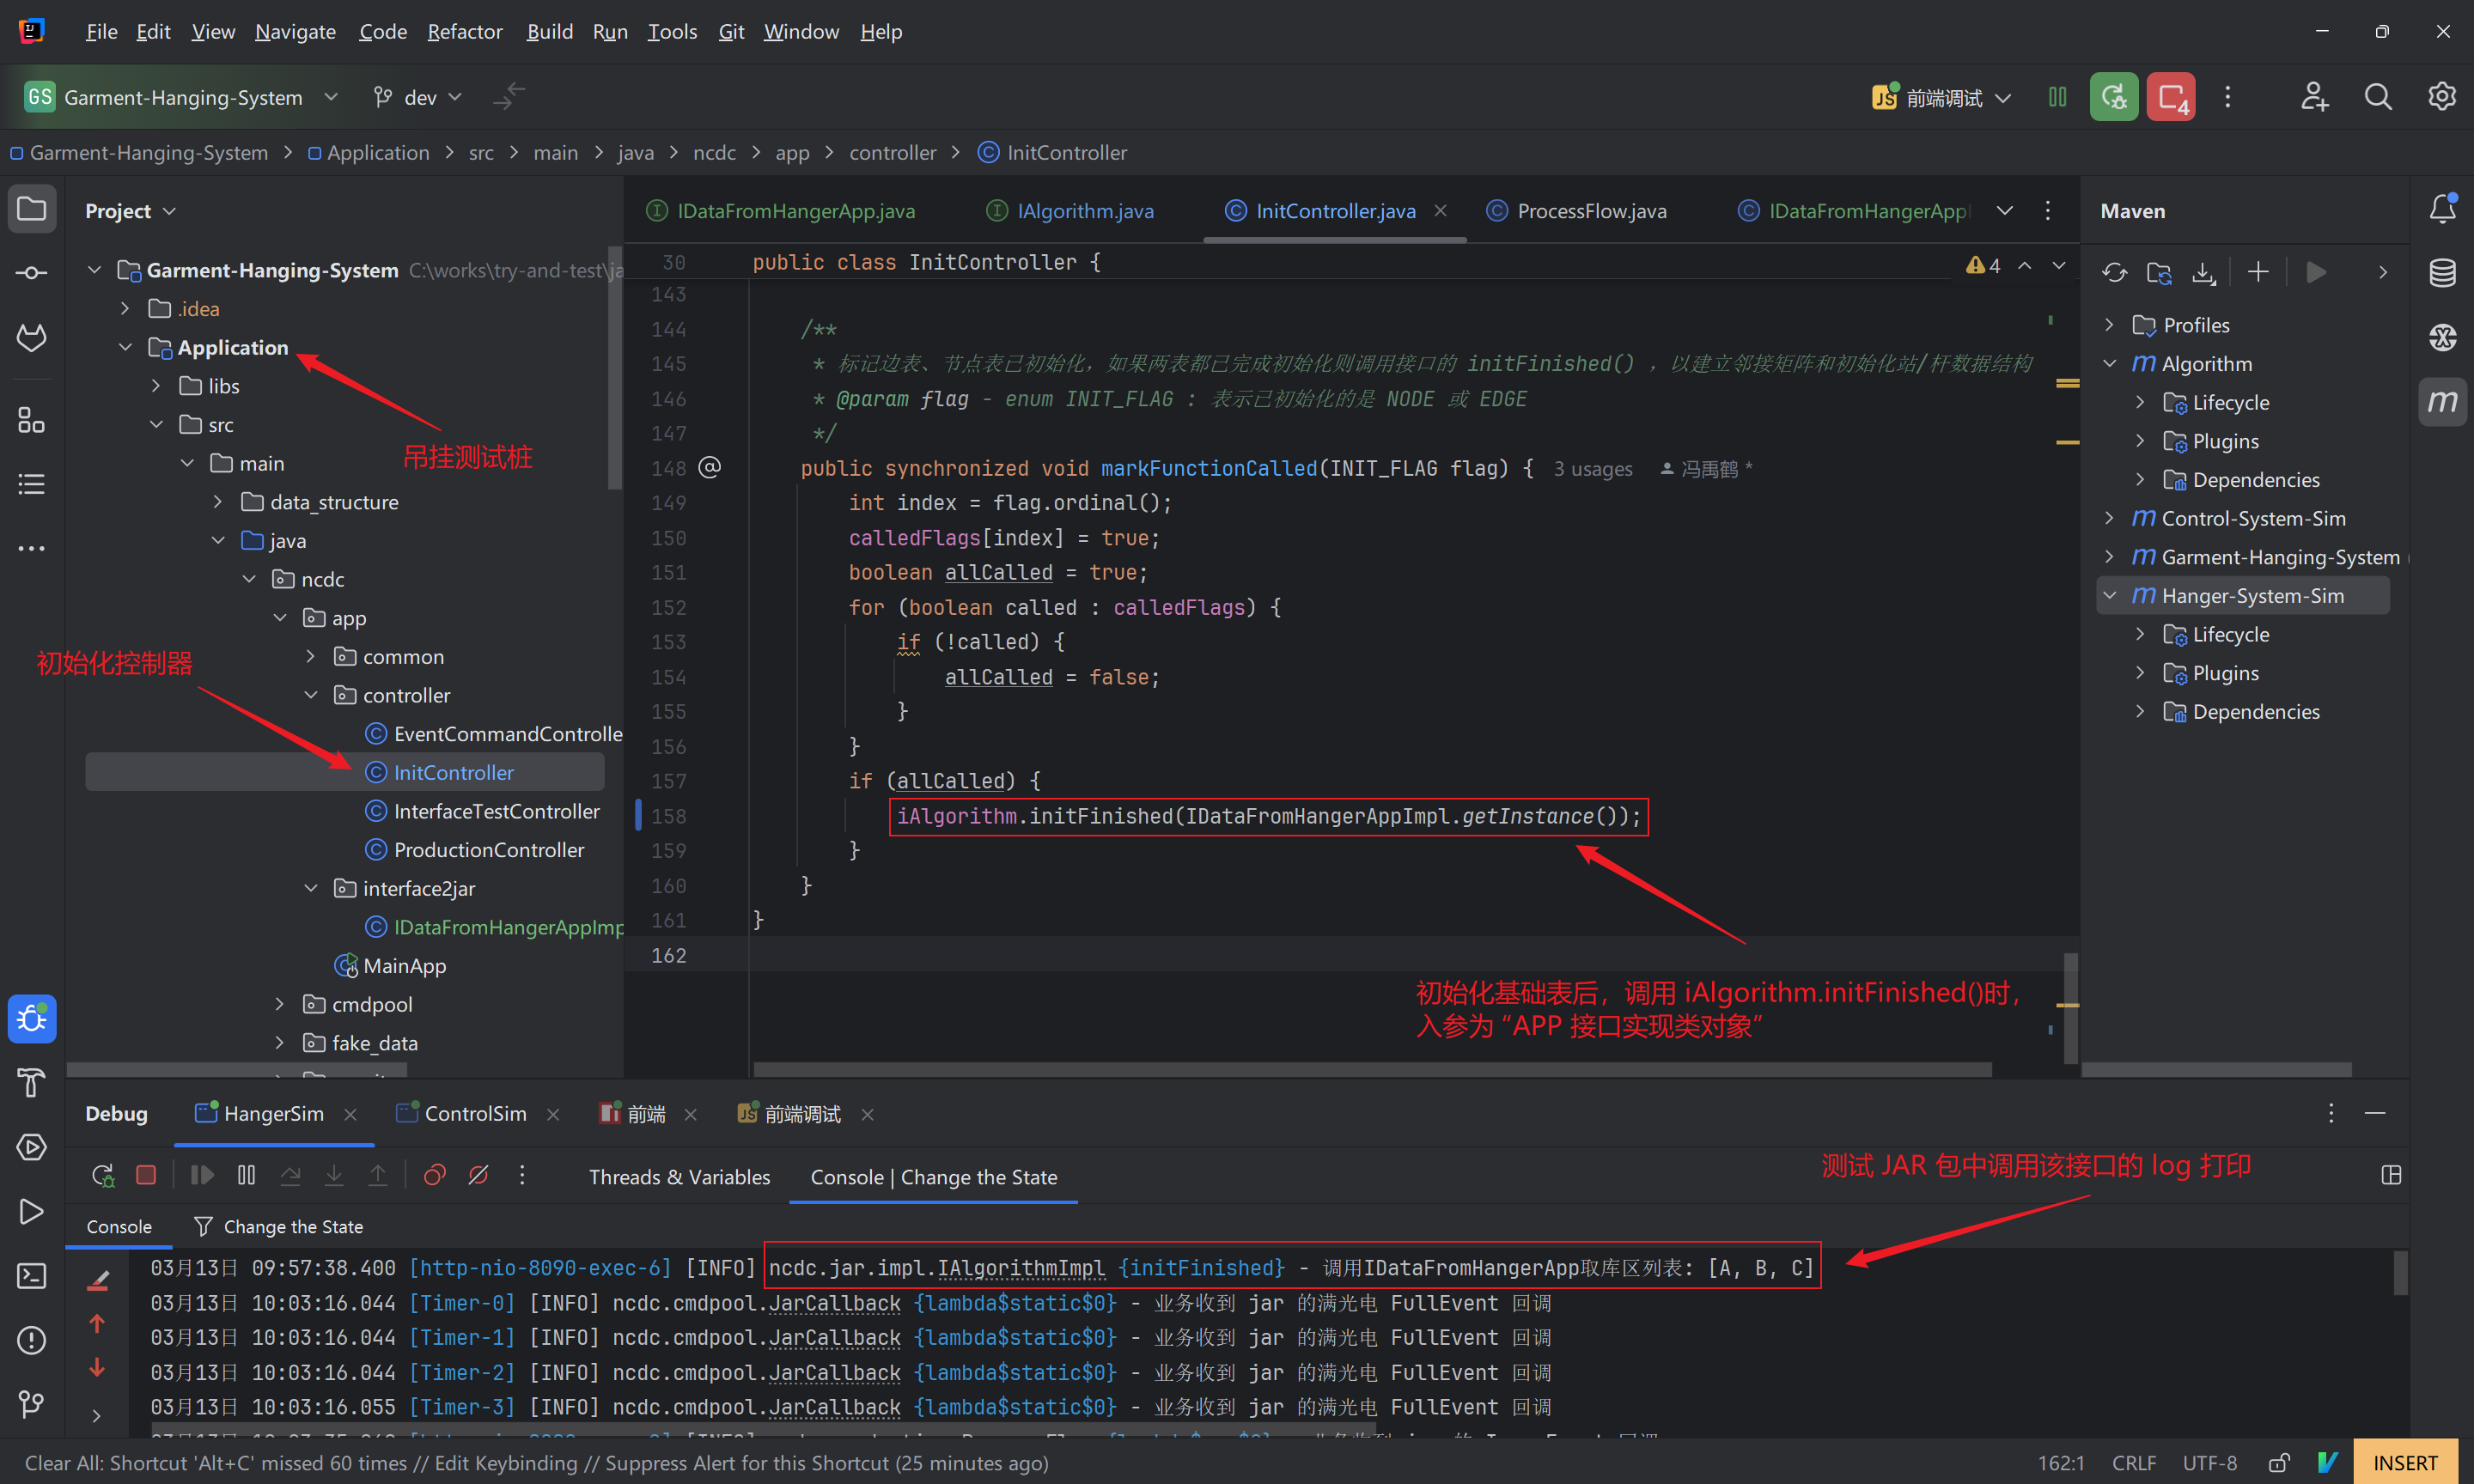
\includegraphics[width=0.8\textwidth]{pics/jack/IDataFromHangerAppImpl.png}
		\caption{APP将接口实现类对象传递给JAR}\label{fig:IDataFromHangerAppImpl}
	\end{figure}
	\tips{新的仓规则方案可能不需要传基础数据给JAR，则可在其它地方传递\bf{该接口实现类对象}给JAR包}。

	\item \bf{测试JAR中调用接口}
	\begin{figure}[H]%[htbp!]
		\centering
		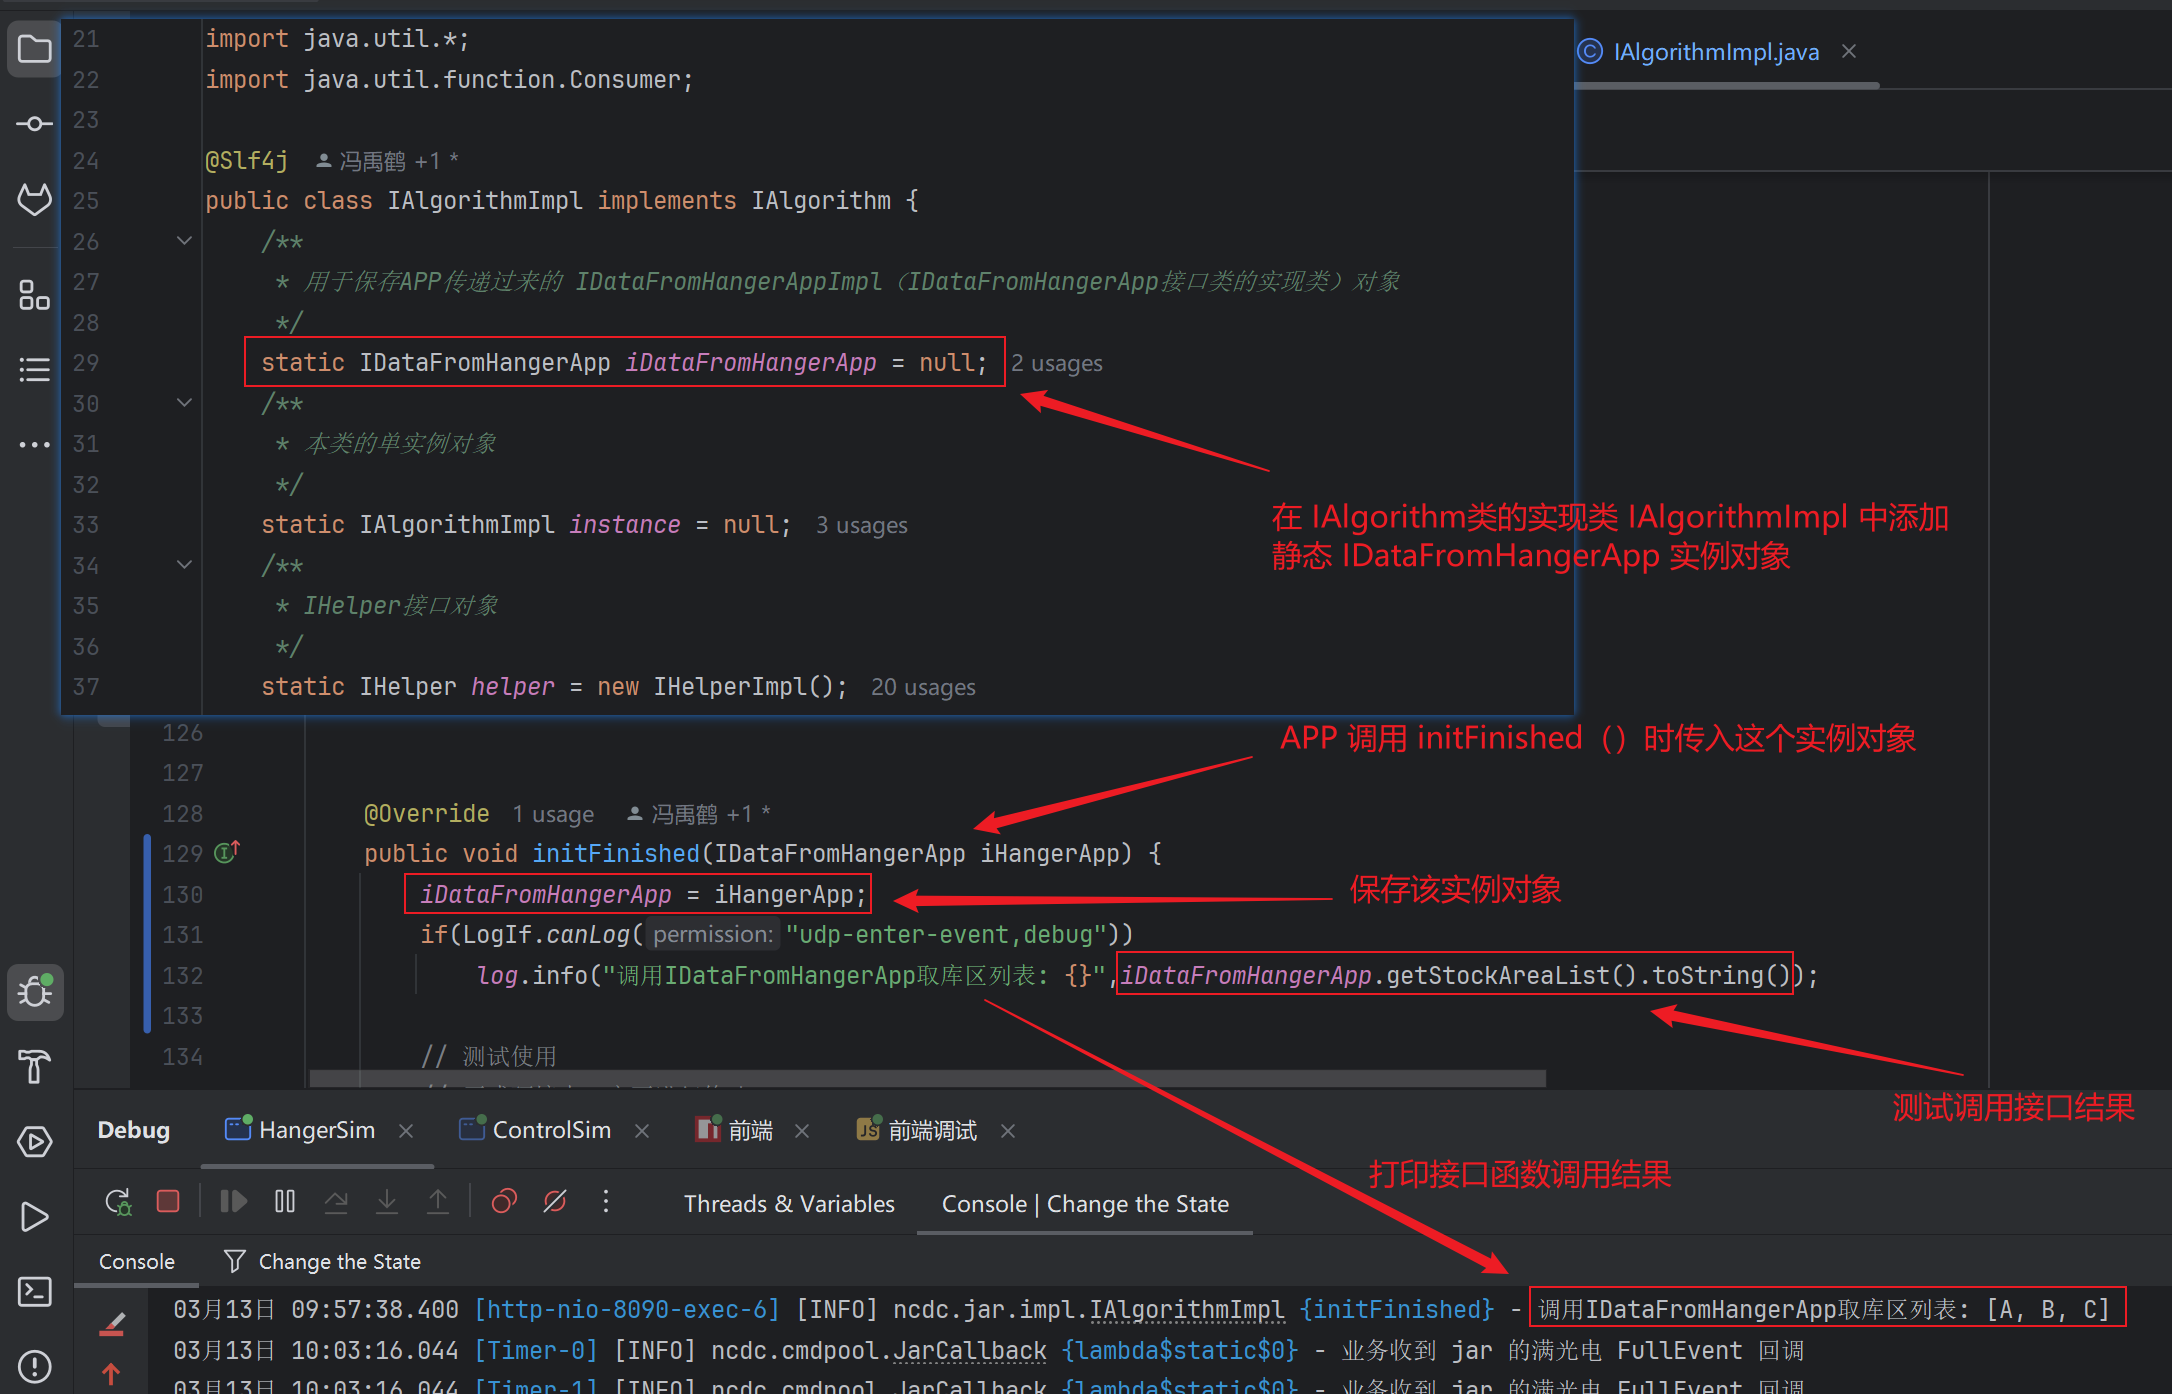
\includegraphics[width=0.8\textwidth]{pics/jack/IDataFromHangerApp_test.png}
		\caption{测试JAR中调用接口}\label{fig:IDataFromHangerApp_test}
	\end{figure}

\end{enumerate}

\subsection{新构架：Entity-Jar-App}
	\begin{figure}[H]%[htbp!]
		\centering
		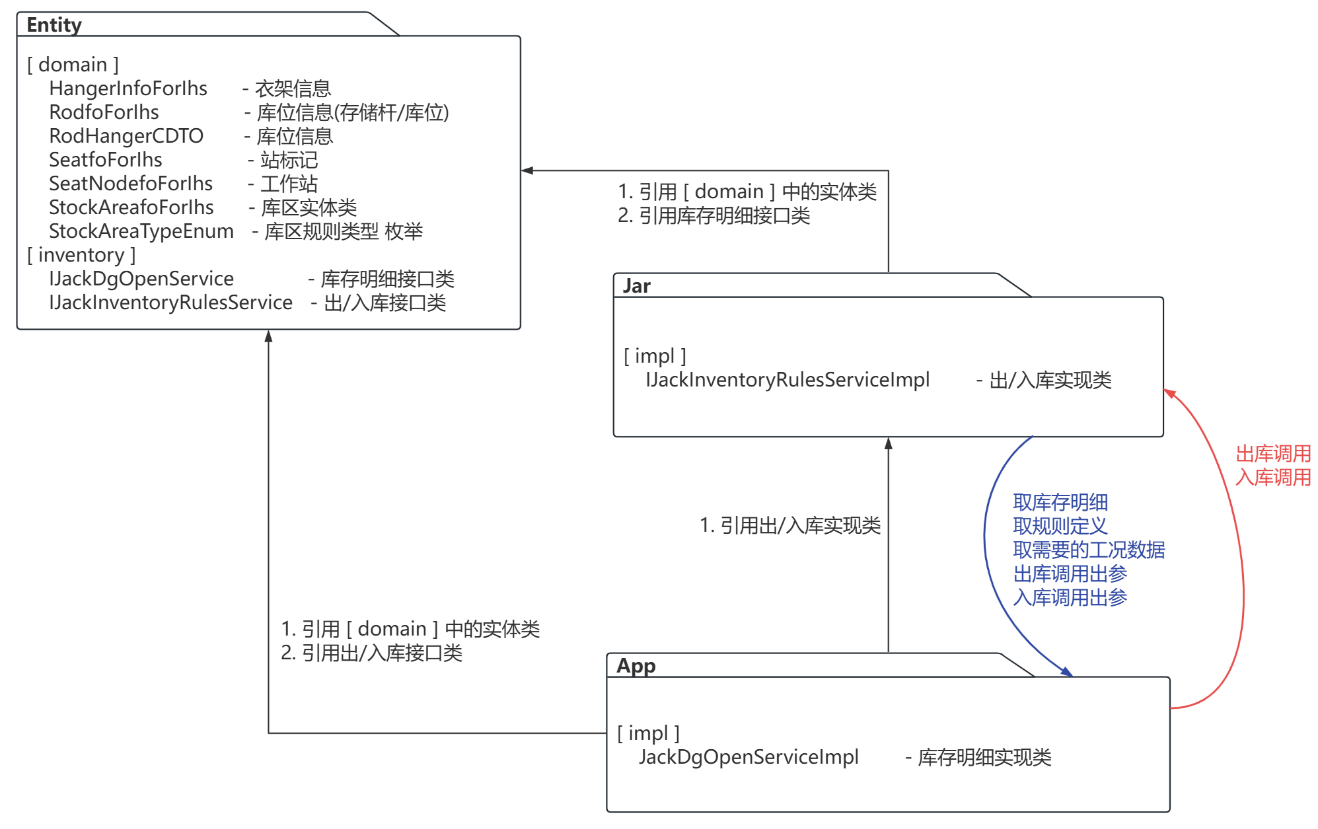
\includegraphics[width=0.8\textwidth]{pics/jack/new-rule-architecture.png}
		\caption{新架构}\label{fig:new-rule-architecture}
	\end{figure}

\subsection{JAR重构}
\begin{enumerate}[label=\arabic*)]
	\item 基础数据移植到APP
	\item 工站、存储杆数据移植到APP
	\item Jar只保留IJackInventoryRulesServiceImpl的实现
	\item Jar临时保留Helper中的几个测试桩（吊挂、控制）使用的类
	\begin{figure}[H]%[htbp!]
		\centering
		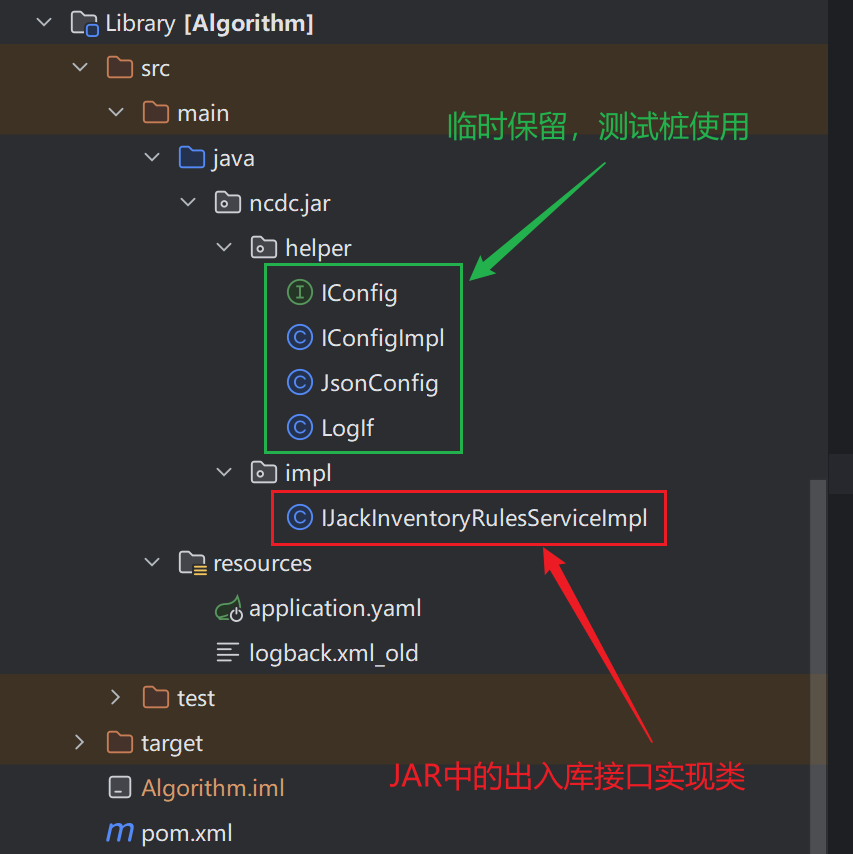
\includegraphics[width=0.35\textwidth]{pics/jack/jar-refactor.png}
		\caption{重构后的Jar包文件}\label{fig:jar-refactor}
	\end{figure}
\end{enumerate}

\subsection{出入库出入参定义及算法工作原理}
\subsubsection{仓类型和基本特点}
\begin{enumerate}[label=\arabic*)]
	\item \bf{各类型仓的规则}：
	\begin{itemize}
		\item 成品仓：
		\item 半成品仓：
		\item 裁片仓：
		\item 空衣架存储仓：
		\item 包装仓：
		\item 外发仓：
	\end{itemize}
	\tips{规则及约束条件，见《吊挂仓需求（功能点）.pdf》}
	\item \bf{各类型仓的业务形态}：
	\begin{itemize}
		\item 小单快反
		\item 大货
	\end{itemize}
\end{enumerate}
\clearpage
\subsubsection{入库出入参}
\begin{lstlisting}
    /**
     * 入库接口 - 从 rods 中选出一个库位
     * @param hangerId - String : 衣架id
     * @param rods - List˂String˃ : 可入库的库位集合
     * @param props - LinkedHashMap˂String, String˃ : 规则属性表，按优先级从高到低构建此参数。Key 可能的范围有: 款式、颜色、尺码、PO、排产单、工序、制单、款号、流水线号
     * @param maxMixture - int : 最大混合度
     * @return - String : 库位
     */
    String inBound(String hangerId, List<String> rods, LinkedHashMap<String, String> props, int maxMixture);
\end{lstlisting}
\begin{itemize}
	\item \bf{入参}
	\begin{enumerate}[label=\arabic*)]
		\item String \it{hangerId}: \bf{衣架ID（衣架信息）} - 可通过此ID获取衣架信息: 包括排产单、\bf{工序}\footnote{\bf{工序}：目前主要是从工序纬度判断混合度}、款/色/码、当前位置等。
		\item List<String> \it{rods}: \bf{库位集合} - 入库可选的存储杆列表
		\item LinkedHashMap<String, String> \it{props}: \bf{Unit类型} - Key可能的范围有: 款式、颜色、尺码、PO、排产单、工序、制单、款号、流水线号
		\item int \it{maxMixture}: \bf{最大混合度} - 意思是与分拣之前的混合度是同一个概念，及一根存储杆上的Unit类型是“款色码”，例如值是：3，disintct（款色码）的个数就是3  
	\end{enumerate}
	\item \bf{出参}
	\begin{enumerate}[label=\arabic*)]
		\item String \it{rod}: \bf{库位}
	\end{enumerate}
\end{itemize}
\begin{figure}[H]%[htbp!]
	\centering
	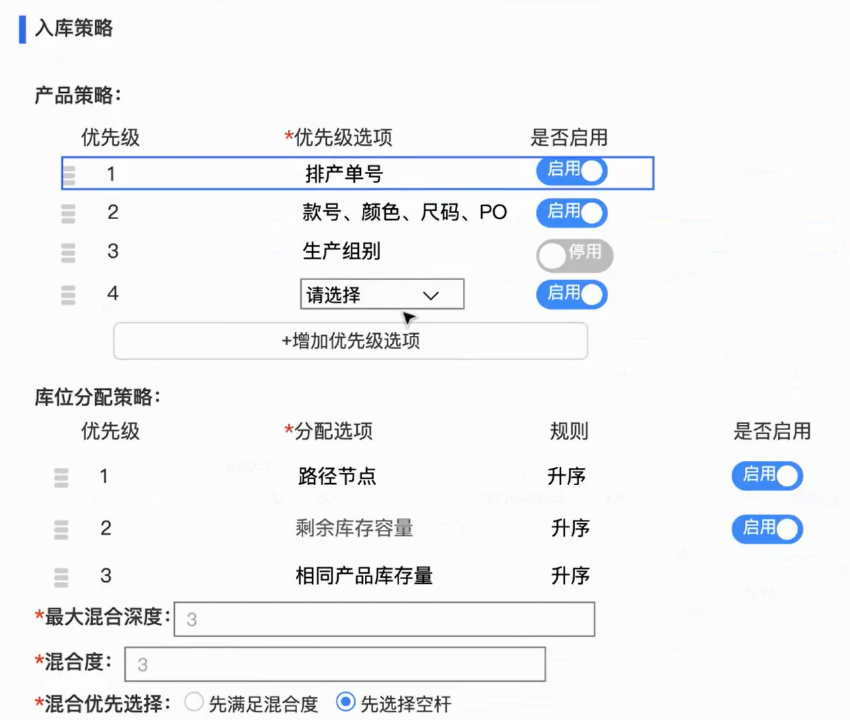
\includegraphics[width=0.45\textwidth]{pics/jack/inbound-rule.png}
	\caption{入库策略前端配置页面}\label{fig:inbound-rule}
\end{figure}

\clearpage
\subsubsection{入库工作原理及基础算法}
\begin{verbatim}
public String inBound(String hangerId, List<String> rods, LinkedHashMap<String, String> props, int maxMixture)
\end{verbatim}
\begin{enumerate}[leftmargin=32pt,label=\bf{步骤\Roman*.}]
	\item \it{空衣架入仓}
	\begin{figure*}[!h]
		\centering
		\resizebox{0.6\linewidth}{!}{\input{out/uml/jack/inBound1/inBound1.latex}}
		\caption{入库算法步骤1}\label{fig:inbound1}
	\end{figure*}
	\par
	空衣架入库规则比较简单，按存储杆列表顺序（rods）直接从可入库的存储杆中选一个即可。可入库的存储杆是指：满光电状态为\it{未满}，且库位衣架数加在途衣架数小于库位容量。
	\item \it{计算备选库位数据}\par
	\bf{方法}：将可用存储杆的\it{库位混存数据}存入备选杆哈希表: $Map<String, MixedInfo> mapCandidateRods$。\bf{可用存储杆}，是 rods 中排除了满光电状态为\it{满}、以及\it{在杆+在途>=容量}的存储杆。\bf{库位混存数据}包括\it{入参属性适配衣架数量}、\it{混存度}，该数据通过遍历存储杆中所有衣架的属性值计算得出。混存度的计算：取出存储杆的入参 props 中属性\footnote{\bf{入参属性}: props, key为\it{款式、颜色、尺码、PO、排产单、工序、制单、款号、流水线号}的子集。}对应的值，按 props 属性顺序将这些值用“$\_$”连接起来得到一个字符串，作为混存度的判断依据。具体是使用一个辅助哈希表：$Map<String, Integer>$ mapMixedDegree，属性值用“$\_$”连接的字符串作为 key ，value为匹配该key的衣架的数量，同时统计与入库算法入参props的key匹配的衣架数。当前杆的衣架遍历结束，就可以得到这两个数据：\cnumm{1} 入参属性适配衣架数量、\cnumm{2} 混存度（key数量），并用这两个数创建\it{MixedInfo}对象，以当前杆号为 key、MixedInfo为 value，添加到mapCandidateRods。这样就为入库算法的下一步做好了准备。\par
	\bf{找到不混存的存储杆}: 遍历存储杆过程中，每迭代一个存储杆结束（迭代下一个存储杆前），当混存度为1且衣架全是入参属性值匹配的衣架时，返回当前杆。\par
	\bf{找到空杆}: 遍历完全部存储杆时，如果发现有空杆，则返回空杆。\par
	\bf{找混存杆}: 见后续步骤“筛选适合的混存杆”。\par
	具体的实现流程见图\ref{fig:inbound2}
	\begin{figure*}[!h]
		\centering
		\resizebox{1.0\linewidth}{!}{\input{out/uml/jack/inBound2/inBound2.latex}}
		\caption{入库算法步骤2}\label{fig:inbound2}
	\end{figure*}
	\item \it{筛选适合的混存杆}\par
	在\it{计算备选库位数据}算法得到的mapCandidateRods基础上，采用如图\ref{fig:inbound3}所示的方法筛选出适合的混存杆。
	\begin{figure*}[!h]
		\centering
		\resizebox{0.8\linewidth}{!}{\input{out/uml/jack/inBound3/inBound3.latex}}
		\caption{入库算法步骤3}\label{fig:inbound3}
	\end{figure*}

\end{enumerate}

\clearpage
\subsubsection{入库算法增强考虑按属性顺序优先}
\begin{enumerate}[leftmargin=32pt,label=\bf{增强\Roman*.}]
	\item \bf{广度优先} 
	\begin{itemize}
		\item \it{策略}: 找同属性衣架的杆$\longrightarrow$ 找空杆  $\longrightarrow$ 找未超出混存度上限的杆
		\item \it{特点}: 靠前的杆混存度高，靠后的杆混存度低，如图\ref{fig:inbound-rule-width-first}所示
		\begin{figure}[H]%[htbp!]
			\centering
			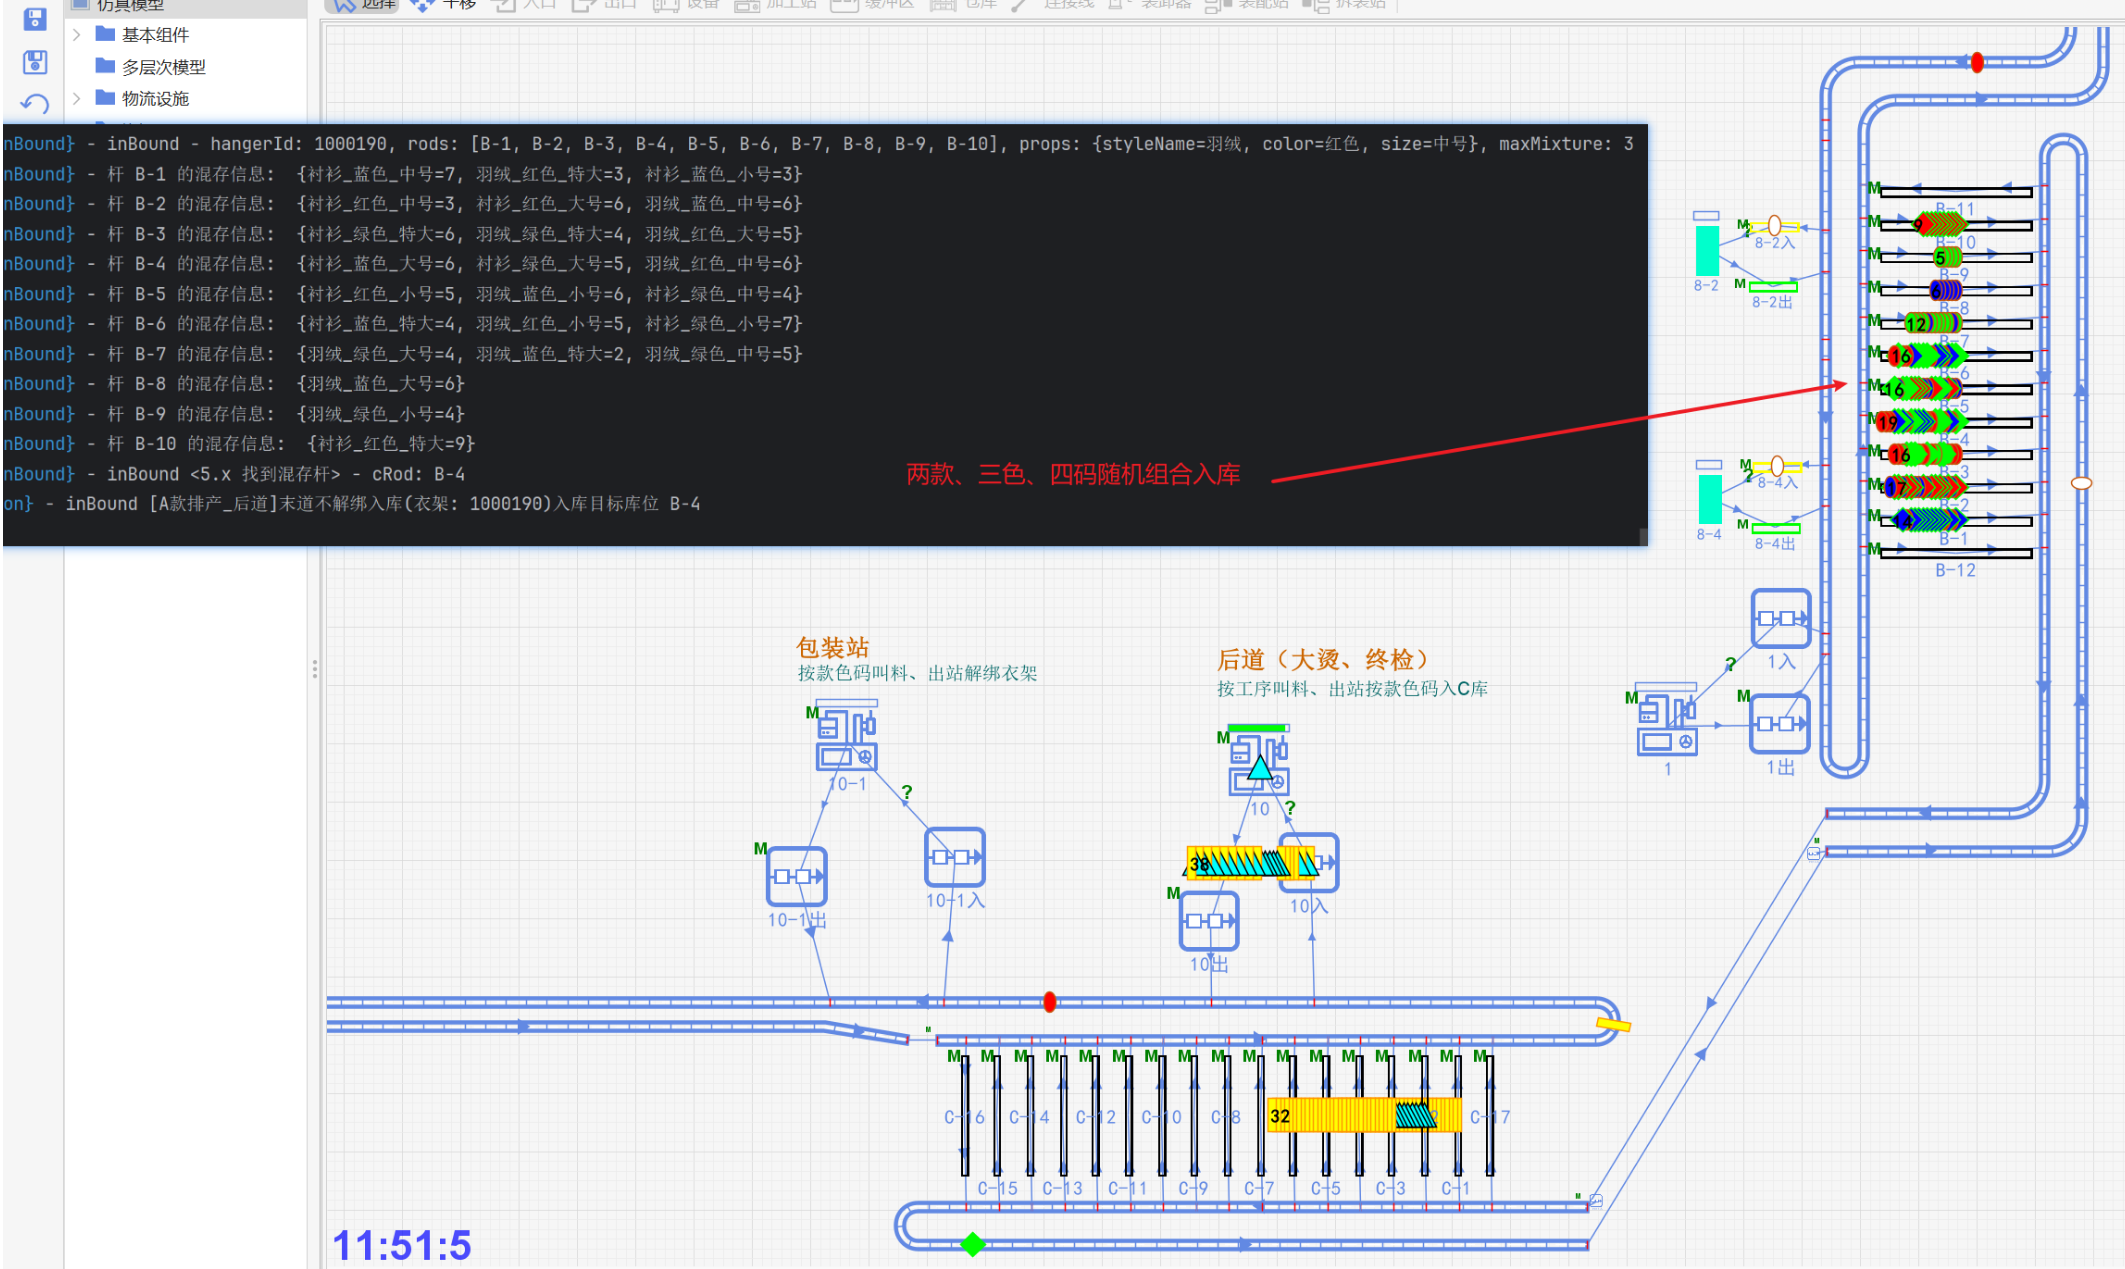
\includegraphics[width=0.8\textwidth]{pics/jack/inbound-rule-width-first.png}
			\caption{入库策略-广度优先}\label{fig:inbound-rule-width-first}
		\end{figure}
	\end{itemize} 
	\item \bf{深度优先【基础算法中默认】}
	\begin{itemize}
		\item \it{策略}: 找同属性衣架的杆$\longrightarrow$ 找空杆  $\longrightarrow$ 找未超出混存度上限的，且混存度相对小的杆
		\item \it{特点}: 可选杆的混存度较均衡，如图\ref{fig:inbound-rule-depth-first}所示
		\begin{figure}[H]%[htbp!]
			\centering
			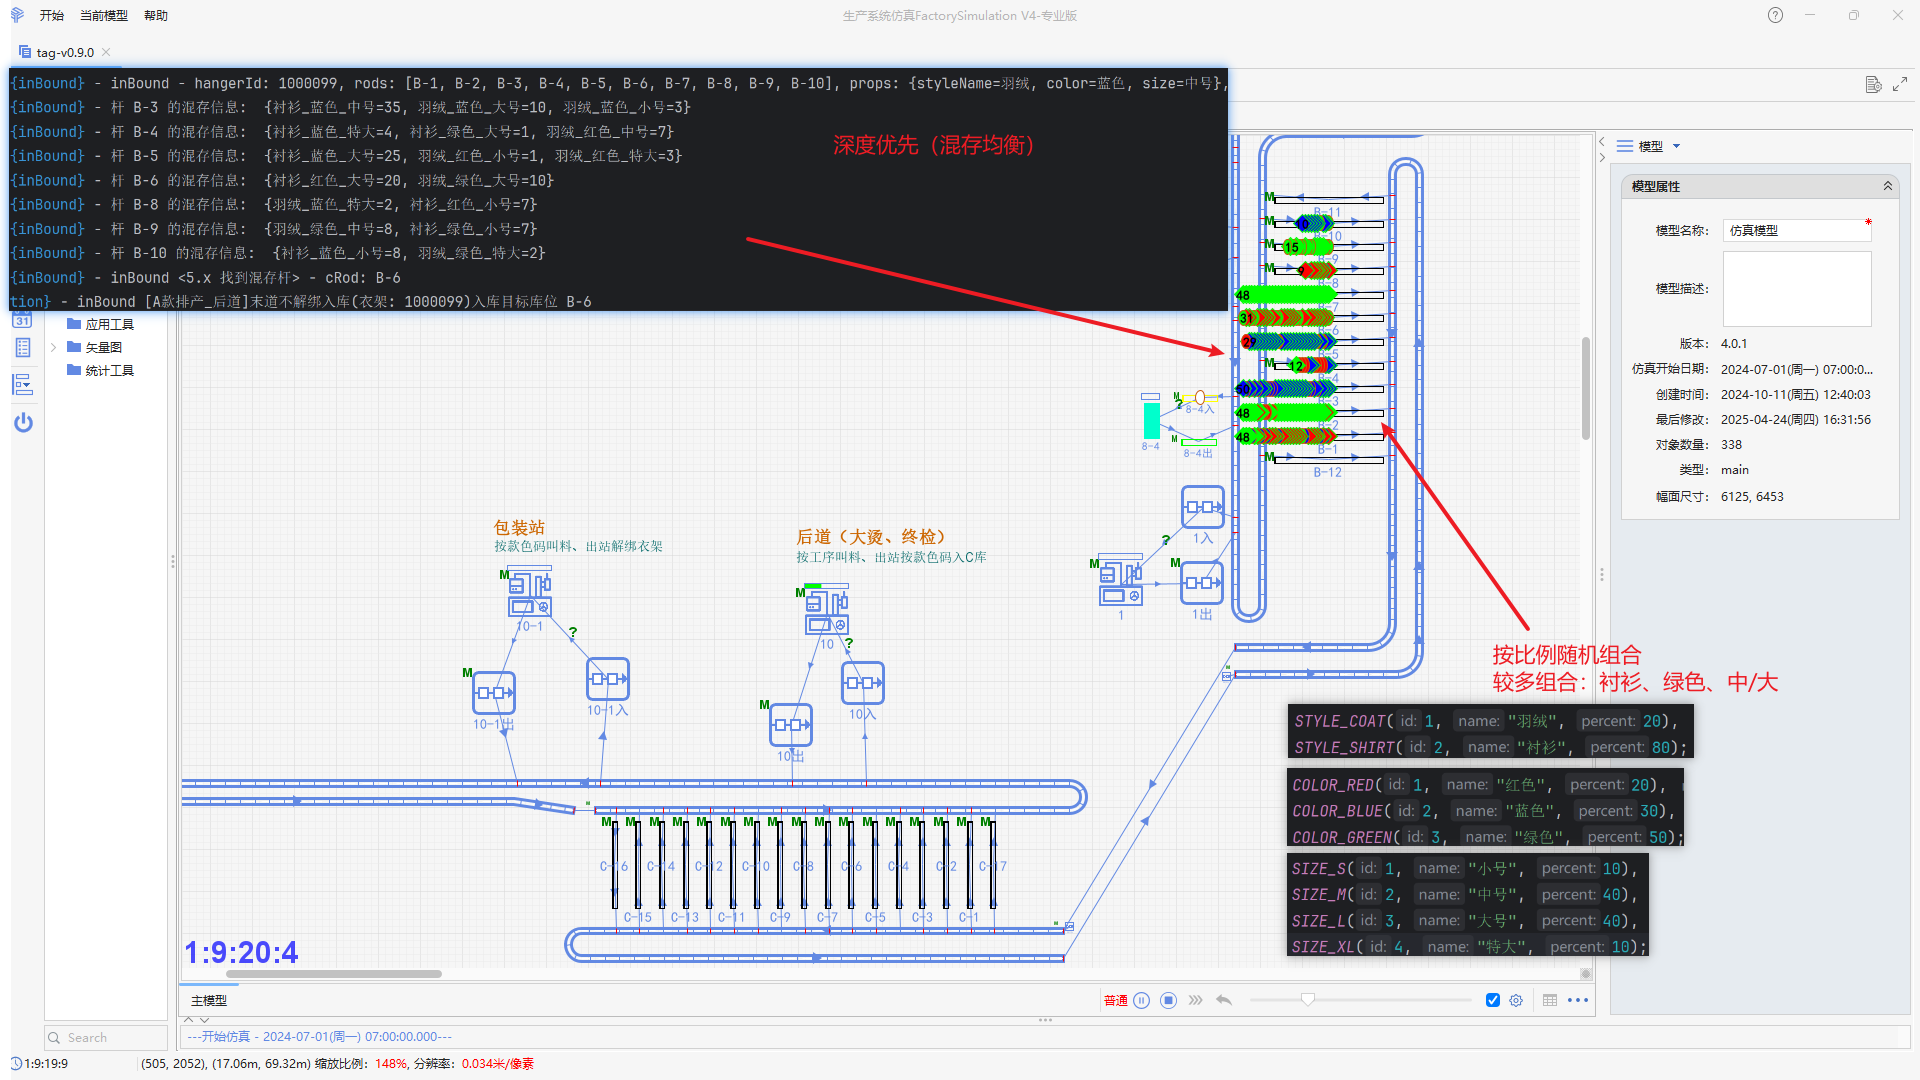
\includegraphics[width=0.8\textwidth]{pics/jack/inbound-rule-depth-first.png}
			\caption{入库策略-深度优先}\label{fig:inbound-rule-depth-first}
		\end{figure}
	\end{itemize} 
	\item \bf{考虑属性优先级【基础算法中默认】}
	\begin{itemize}
		\item \it{策略}: 找同属性衣架的杆$\longrightarrow$ 找空杆  $\longrightarrow$ 找未超出混存度上限的，且更粗颗粒度匹配的杆 $\longrightarrow$ 找未超出混存度上限的，且混存度相对小的杆
		\item \it{方法}: 在第二步\bf{计算备选库位数据}时，按入参props的顺序逐步划分颗粒度（也即混存深度）\footnote{\bf{颗粒度 vs.混存深度}：props的属性个数越多，颗粒度越细，混存深度越大。入参props的属性排前的属性颗粒度粗。不考虑属性优先级时，props的属性在先在后对库位筛选没有影响。}，例如按“款、色、码”为属性，颗粒度由粗到细，依次是“款”、“款\_色”、“款\_色\_码”。在选择杆时，未命中细颗粒度的杆时，要选择某杆混存，优先选粗颗粒度命中的杆。以下是衣架\it{1000335}入库时的日志信息，更多的日志信息见\ref{sec:inbound-log}节。
		{\scriptsize
		\begin{verbatim}
{inBound} - hangerId: 1000335, rods: [B-1, B-2, B-3, B-4, B-5, B-6, B-7, B-8, B-9, B-10], props: {styleName=衬衫, color=绿色, size=中号}, 
            maxMixture: 3
{inBound} - 杆 B-1 的混存信息（最细）:  {衬衫_绿色_大号=6, 羽绒_蓝色_中号=2}
{inBound} - 杆 B-1 的混存信息（全部）:  {
		1=MixedData(countMatchedProps=6, mixedDegree=2, mapMixedDegree={羽绒=2, 衬衫=6}), 
		2=MixedData(countMatchedProps=6, mixedDegree=2, mapMixedDegree={衬衫_绿色=6, 羽绒_蓝色=2}), 
		3=MixedData(countMatchedProps=0, mixedDegree=2, mapMixedDegree={衬衫_绿色_大号=6, 羽绒_蓝色_中号=2})}
{inBound} - 杆 B-2 的混存信息（最细）:  {衬衫_红色_特大=1, 衬衫_绿色_特大=2}
{inBound} - 杆 B-2 的混存信息（全部）:  {
		1=MixedData(countMatchedProps=3, mixedDegree=1, mapMixedDegree={衬衫=3}), 
		2=MixedData(countMatchedProps=2, mixedDegree=2, mapMixedDegree={衬衫_绿色=2, 衬衫_红色=1}), 
		3=MixedData(countMatchedProps=0, mixedDegree=2, mapMixedDegree={衬衫_红色_特大=1, 衬衫_绿色_特大=2})}
{inBound} - 杆 B-3 的混存信息（最细）:  {衬衫_蓝色_中号=2, 衬衫_绿色_中号=4}
{inBound} - 杆 B-3 的混存信息（全部）:  {
		1=MixedData(countMatchedProps=6, mixedDegree=1, mapMixedDegree={衬衫=6}), 
		2=MixedData(countMatchedProps=4, mixedDegree=2, mapMixedDegree={衬衫_绿色=4, 衬衫_蓝色=2}), 
		3=MixedData(countMatchedProps=4, mixedDegree=2, mapMixedDegree={衬衫_蓝色_中号=2, 衬衫_绿色_中号=4})}
{inBound} - 杆 B-4 的混存信息（最细）:  {衬衫_红色_中号=3, 衬衫_红色_小号=1}
{inBound} - 杆 B-4 的混存信息（全部）:  {
		1=MixedData(countMatchedProps=4, mixedDegree=1, mapMixedDegree={衬衫=4}), 
		2=MixedData(countMatchedProps=0, mixedDegree=1, mapMixedDegree={衬衫_红色=4}), 
		3=MixedData(countMatchedProps=0, mixedDegree=2, mapMixedDegree={衬衫_红色_中号=3, 衬衫_红色_小号=1})}
{inBound} - 杆 B-5 的混存信息（最细）:  {衬衫_绿色_小号=2}
{inBound} - 杆 B-5 的混存信息（全部）:  {
		1=MixedData(countMatchedProps=2, mixedDegree=1, mapMixedDegree={衬衫=2}), 
		2=MixedData(countMatchedProps=2, mixedDegree=1, mapMixedDegree={衬衫_绿色=2}), 
		3=MixedData(countMatchedProps=0, mixedDegree=1, mapMixedDegree={衬衫_绿色_小号=2})}
{inBound} - 杆 B-6 的混存信息（最细）:  {羽绒_绿色_中号=2}
{inBound} - 杆 B-6 的混存信息（全部）:  {
		1=MixedData(countMatchedProps=0, mixedDegree=1, mapMixedDegree={羽绒=2}), 
		2=MixedData(countMatchedProps=0, mixedDegree=1, mapMixedDegree={羽绒_绿色=2}), 
		3=MixedData(countMatchedProps=0, mixedDegree=1, mapMixedDegree={羽绒_绿色_中号=2})}
{inBound} - 杆 B-7 的混存信息（最细）:  {衬衫_红色_大号=4}
{inBound} - 杆 B-7 的混存信息（全部）:  {
		1=MixedData(countMatchedProps=4, mixedDegree=1, mapMixedDegree={衬衫=4}), 
		2=MixedData(countMatchedProps=0, mixedDegree=1, mapMixedDegree={衬衫_红色=4}), 
		3=MixedData(countMatchedProps=0, mixedDegree=1, mapMixedDegree={衬衫_红色_大号=4})}
{inBound} - 杆 B-8 的混存信息（最细）:  {衬衫_蓝色_大号=4}
{inBound} - 杆 B-8 的混存信息（全部）:  {
		1=MixedData(countMatchedProps=4, mixedDegree=1, mapMixedDegree={衬衫=4}), 
		2=MixedData(countMatchedProps=0, mixedDegree=1, mapMixedDegree={衬衫_蓝色=4}), 
		3=MixedData(countMatchedProps=0, mixedDegree=1, mapMixedDegree={衬衫_蓝色_大号=4})}
{inBound} - 杆 B-9 的混存信息（最细）:  {羽绒_绿色_大号=1}
{inBound} - 杆 B-9 的混存信息（全部）:  {
		1=MixedData(countMatchedProps=0, mixedDegree=1, mapMixedDegree={羽绒=1}), 
		2=MixedData(countMatchedProps=0, mixedDegree=1, mapMixedDegree={羽绒_绿色=1}), 
		3=MixedData(countMatchedProps=0, mixedDegree=1, mapMixedDegree={羽绒_绿色_大号=1})}
{inBound} - 杆 B-10 的混存信息（最细）:  {羽绒_红色_中号=1
{inBound} - 杆 B-10 的混存信息（全部）:  {
		1=MixedData(countMatchedProps=0, mixedDegree=1, mapMixedDegree={羽绒=1}), 
		2=MixedData(countMatchedProps=0, mixedDegree=1, mapMixedDegree={羽绒_红色=1}), 
		3=MixedData(countMatchedProps=0, mixedDegree=1, mapMixedDegree={羽绒_红色_中号=1})}
{inBound} <5.x 找到混存杆> - cRod: B-3
<=== [A款排产_后道]末道不解绑入库(衣架: 1000335)入库目标库位 B-3
		\end{verbatim}
		}
		日志分析：
		\begin{itemize}
			\item \it{入参}: 衣架1000335的款式、颜色、尺码分别是“衬衫”、“绿色”、“中号”，最大混存度允许3。
			\item \it{混存深度1}：入参属性选择\bf{衬衫}，各杆的匹配情况为：
			\begin{itemize}
				\item \bf{B-1}:  匹配\it{6}个衣架，混存度2（羽绒=2, 衬衫=6）
				\item \bf{B-2}:  匹配\it{3}个衣架，混存度1（衬衫=3）
				\item \bf{B-3}:  匹配\it{6}个衣架，混存度1（衬衫=6）
				\item \bf{B-4}:  匹配\it{4}个衣架，混存度1（衬衫=4）
				\item \bf{B-5}:  匹配\it{2}个衣架，混存度1（衬衫=2）
				\item \bf{B-6}:  匹配\it{0}个衣架，混存度1（羽绒=2）
				\item \bf{B-7}:  匹配\it{4}个衣架，混存度1（衬衫=4）
				\item \bf{B-8}:  匹配\it{4}个衣架，混存度1（衬衫=4）
				\item \bf{B-9}:  匹配\it{0}个衣架，混存度1（羽绒=1）
				\item \bf{B-10}: 匹配\it{0}个衣架，混存度1（羽绒=1）
			\end{itemize}
			\item \it{混存深度2}：入参属性选择\bf{衬衫\_绿色}，各杆的匹配情况为：
			\begin{itemize}
				\item \bf{B-1}:  匹配\it{6}个衣架，混存度2（衬衫\_绿色=6, 羽绒\_蓝色=2）
				\item \bf{B-2}:  匹配\it{2}个衣架，混存度2（衬衫\_绿色=2, 衬衫\_红色=1）
				\item \bf{B-3}:  匹配\it{4}个衣架，混存度2（衬衫\_绿色=4, 衬衫\_蓝色=2）
				\item \bf{B-4}:  匹配\it{0}个衣架，混存度1（衬衫\_红色=4）
				\item \bf{B-5}:  匹配\it{2}个衣架，混存度1（衬衫\_绿色=2）
				\item \bf{B-6}:  匹配\it{0}个衣架，混存度1（羽绒\_绿色=2）
				\item \bf{B-7}:  匹配\it{0}个衣架，混存度1（衬衫\_红色=4）
				\item \bf{B-8}:  匹配\it{0}个衣架，混存度1（衬衫\_蓝色=4）
				\item \bf{B-9}:  匹配\it{0}个衣架，混存度1（羽绒\_绿色=1）
				\item \bf{B-10}: 匹配\it{0}个衣架，混存度1（羽绒\_红色=1）
			\end{itemize}
			\item \it{混存深度3}：入参属性选择\bf{衬衫\_绿色\_中号}，各杆的匹配情况为：
			\begin{itemize}
				\item \bf{B-1}:  匹配\it{0}个衣架，混存度2（衬衫\_绿色\_大号=6, 羽绒\_蓝色\_中号=2）
				\item \bf{B-2}:  匹配\it{0}个衣架，混存度2（衬衫\_红色\_特大=1, 衬衫\_绿色\_特大=2）
				\item \bf{B-3}:  匹配\it{4}个衣架，混存度2（衬衫\_蓝色\_中号=2, 衬衫\_绿色\_中号=4）
				\item \bf{B-4}:  匹配\it{0}个衣架，混存度2（衬衫\_红色\_中号=3, 衬衫\_红色\_小号=1）
				\item \bf{B-5}:  匹配\it{0}个衣架，混存度1（衬衫\_绿色\_小号=2）
				\item \bf{B-6}:  匹配\it{0}个衣架，混存度1（羽绒\_绿色\_中号=2）
				\item \bf{B-7}:  匹配\it{0}个衣架，混存度1（衬衫\_红色\_大号=4）
				\item \bf{B-8}:  匹配\it{0}个衣架，混存度1（衬衫\_蓝色\_大号=4）
				\item \bf{B-9}:  匹配\it{0}个衣架，混存度1（羽绒\_绿色\_大号=1）
				\item \bf{B-10}: 匹配\it{0}个衣架，混存度1（羽绒\_红色\_中号=1）
			\end{itemize}
			\item \it{结果}: 由于B-3杆找到入参props的最细颗粒度匹配的衣架，所以选择B-3杆入库。\par

		\end{itemize}
		\item \it{特点}: 以“款、色、码”的取值“衬衫、蓝色、大号”入库为例，库中已存衣架（包括在途）没有找到“衬衫、蓝色、大号”时，尝试找“衬衫、蓝色”的杆，找不到时，再找“衬衫”的杆。
	\end{itemize} 
\end{enumerate}

\clearpage
\subsubsection{出库出入参}
\begin{lstlisting}
    /**
     * 出库接口
     * @param rods - List˂String˃ : 可出库的库位集合
     * @param props - LinkedHashMap˂String, String˃ : 规则属性表，按优先级从高到低构建此参数。Key 可能的范围有: 款式、颜色、尺码、PO、排产单、工序、制单、款号、流水线号
     * @param numberRequest - int : 出库衣架数量
     * @return - Map˂String, List˂String˃˃ : 出库的存储杆及其衣架列表
     */
    Map<String, List<String>> outBound(List<String> rods, LinkedHashMap<String, String> props, int numberRequest );
\end{lstlisting}
\begin{itemize}
	\item \bf{入参}
	\begin{enumerate}[label=\arabic*)]
		\item List<String> \it{rods}: \bf{库位集合} - 出可选的存储杆列表
		\item LinkedHashMap<String, String> \it{props}: \bf{Unit类型} - Key可能的范围有: 款式、颜色、尺码、PO、排产单、工序、制单、款号、流水线号
		\item int \it{numberRequest}: \bf{衣架数量}
	\end{enumerate}
	\item \bf{出参}
	\begin{enumerate}[label=\arabic*)]
		\item Map< String, List<String> > \it{hangersInRods}: \bf{存储杆及其衣架列表} - Key: 存储杆，Value: 衣架列表
	\end{enumerate}
\end{itemize}
\begin{figure}[H]%[htbp!]
	\centering
	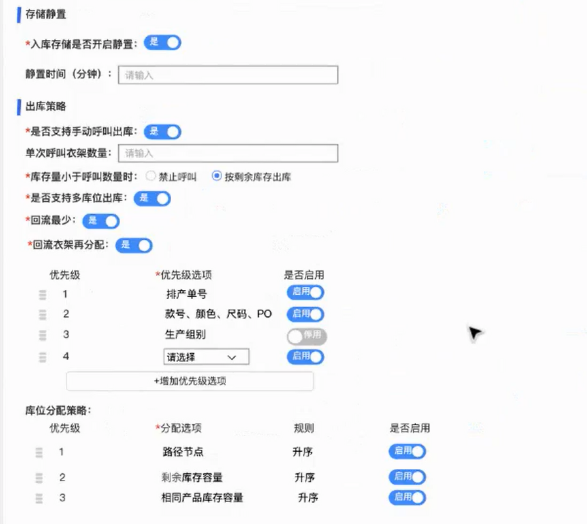
\includegraphics[width=0.45\textwidth]{pics/jack/outbond-rule.png}
	\caption{出库策略前端配置页面}\label{fig:outbound-rule}
\end{figure}

\clearpage
\subsubsection{出库工作原理及算法}
\begin{verbatim}
public Map<String, List<String>> outBound(List<String> rods, LinkedHashMap<String, String> props, int numberRequest)
\end{verbatim}
\begin{enumerate}[leftmargin=32pt,label=\bf{步骤\Roman*.}]
	\item \it{空衣架筛选出库}\par
	如图\ref{fig:outbound1}所示，空衣架出库算法第一步是回调App（吊挂实现的IJackDgOpenService.isEmptyHangerRod(rods.get(0))），因为是空衣架出库，入参rods中任意一个杆都是空衣架存储杆。然后，遍历所有存储杆，回调IJackDgOpenService取该杆是否被预订，回调IJackDgOpenService取在杆衣架数。找到第一个没有被预订，并且有衣架的杆，就是可出库的杆。然后，回调IJackDgOpenService取该杆的衣架列表，创建LinkedHashMap$<$String, List$<$String$>>$出参对象并返回。\par
	\begin{figure*}[!h]
		\centering
		\resizebox{0.8\linewidth}{!}{\input{out/uml/jack/outBound1/outBound1.latex}}
		\caption{出库算法步骤1}\label{fig:outbound1}
	\end{figure*}
	\item \it{求非空衣架出库候选杆数组}\par
	如图\ref{fig:outbound2}所示, 这一步的目的是从\it{入参rods}中分析匹配\it{入参props}衣架有哪些杆，并且这些杆中的匹配衣架在哪个位置开始存放。这些信息用二维数组和一个int型变量表示，二维数组定义和初始化如下：
	\begin{lstlisting}
ArrayList<String>[] blockDegreeRods = new ArrayList[200];
Arrays.setAll(blockDegreeRods, i -> new ArrayList<>());
	\end{lstlisting}
	int型变量保存\it{最大阻挡深度}，也即在遍历rods时，保存衣架最多的杆的衣架数。举例如下：
	{\footnotesize
	\begin{verbatim}
// 2.1 blockDegreeRods(阻挡深度分类存储杆)数组初始化: 按阻挡深度记录找到匹配衣架的杆
//     记录某阻挡深度出现第一个匹配衣架的存储杆（假设存储杆最多存200个衣架, 也即阻挡深度可选0~199）。某深度可以有0~n个杆。
//     blockDegreeRods[0] -> [A-2, A-4]       -- A-2、A-4两杆的第1个衣架就是出库props匹配的衣架，可能第2、3...个衣架也是匹配的，但此处不关心
//     blockDegreeRods[1] -> [A-3]            -- A-3的第2个衣架是匹配衣架
//     blockDegreeRods[2] -> []               -- 所有杆(入参rods)中没有找到第3个衣架是第一个匹配的衣架
//     blockDegreeRods[3] -> [A-5,A-6,A-7]    -- A-5、A-6、A-7的第4个衣架是第一个匹配props的衣架
	\end{verbatim}
	}
	\begin{figure*}[!h]
		\centering
		\resizebox{0.95\linewidth}{!}{\input{out/uml/jack/outBound2/outBound2.latex}}
		\caption{出库算法步骤2}\label{fig:outbound2}
	\end{figure*}
	\clearpage
	\item \it{在阻挡深度分类存储杆中筛选出库衣架}\par
	如图\ref{fig:outbound3}所示。
	\begin{figure*}[!h]
		\centering
		\resizebox{0.6\linewidth}{!}{\input{out/uml/jack/outBound3/outBound3.latex}}
		\caption{出库算法步骤3}\label{fig:outbound3}
	\end{figure*}

\end{enumerate}

\clearpage
\subsubsection{增加按款色码出入库策略}
\begin{enumerate}[label=\arabic*)]
	\item \bf{FS模型修改}
	\begin{itemize}
		\begin{figure}[H]%[htbp!]
			\centering
			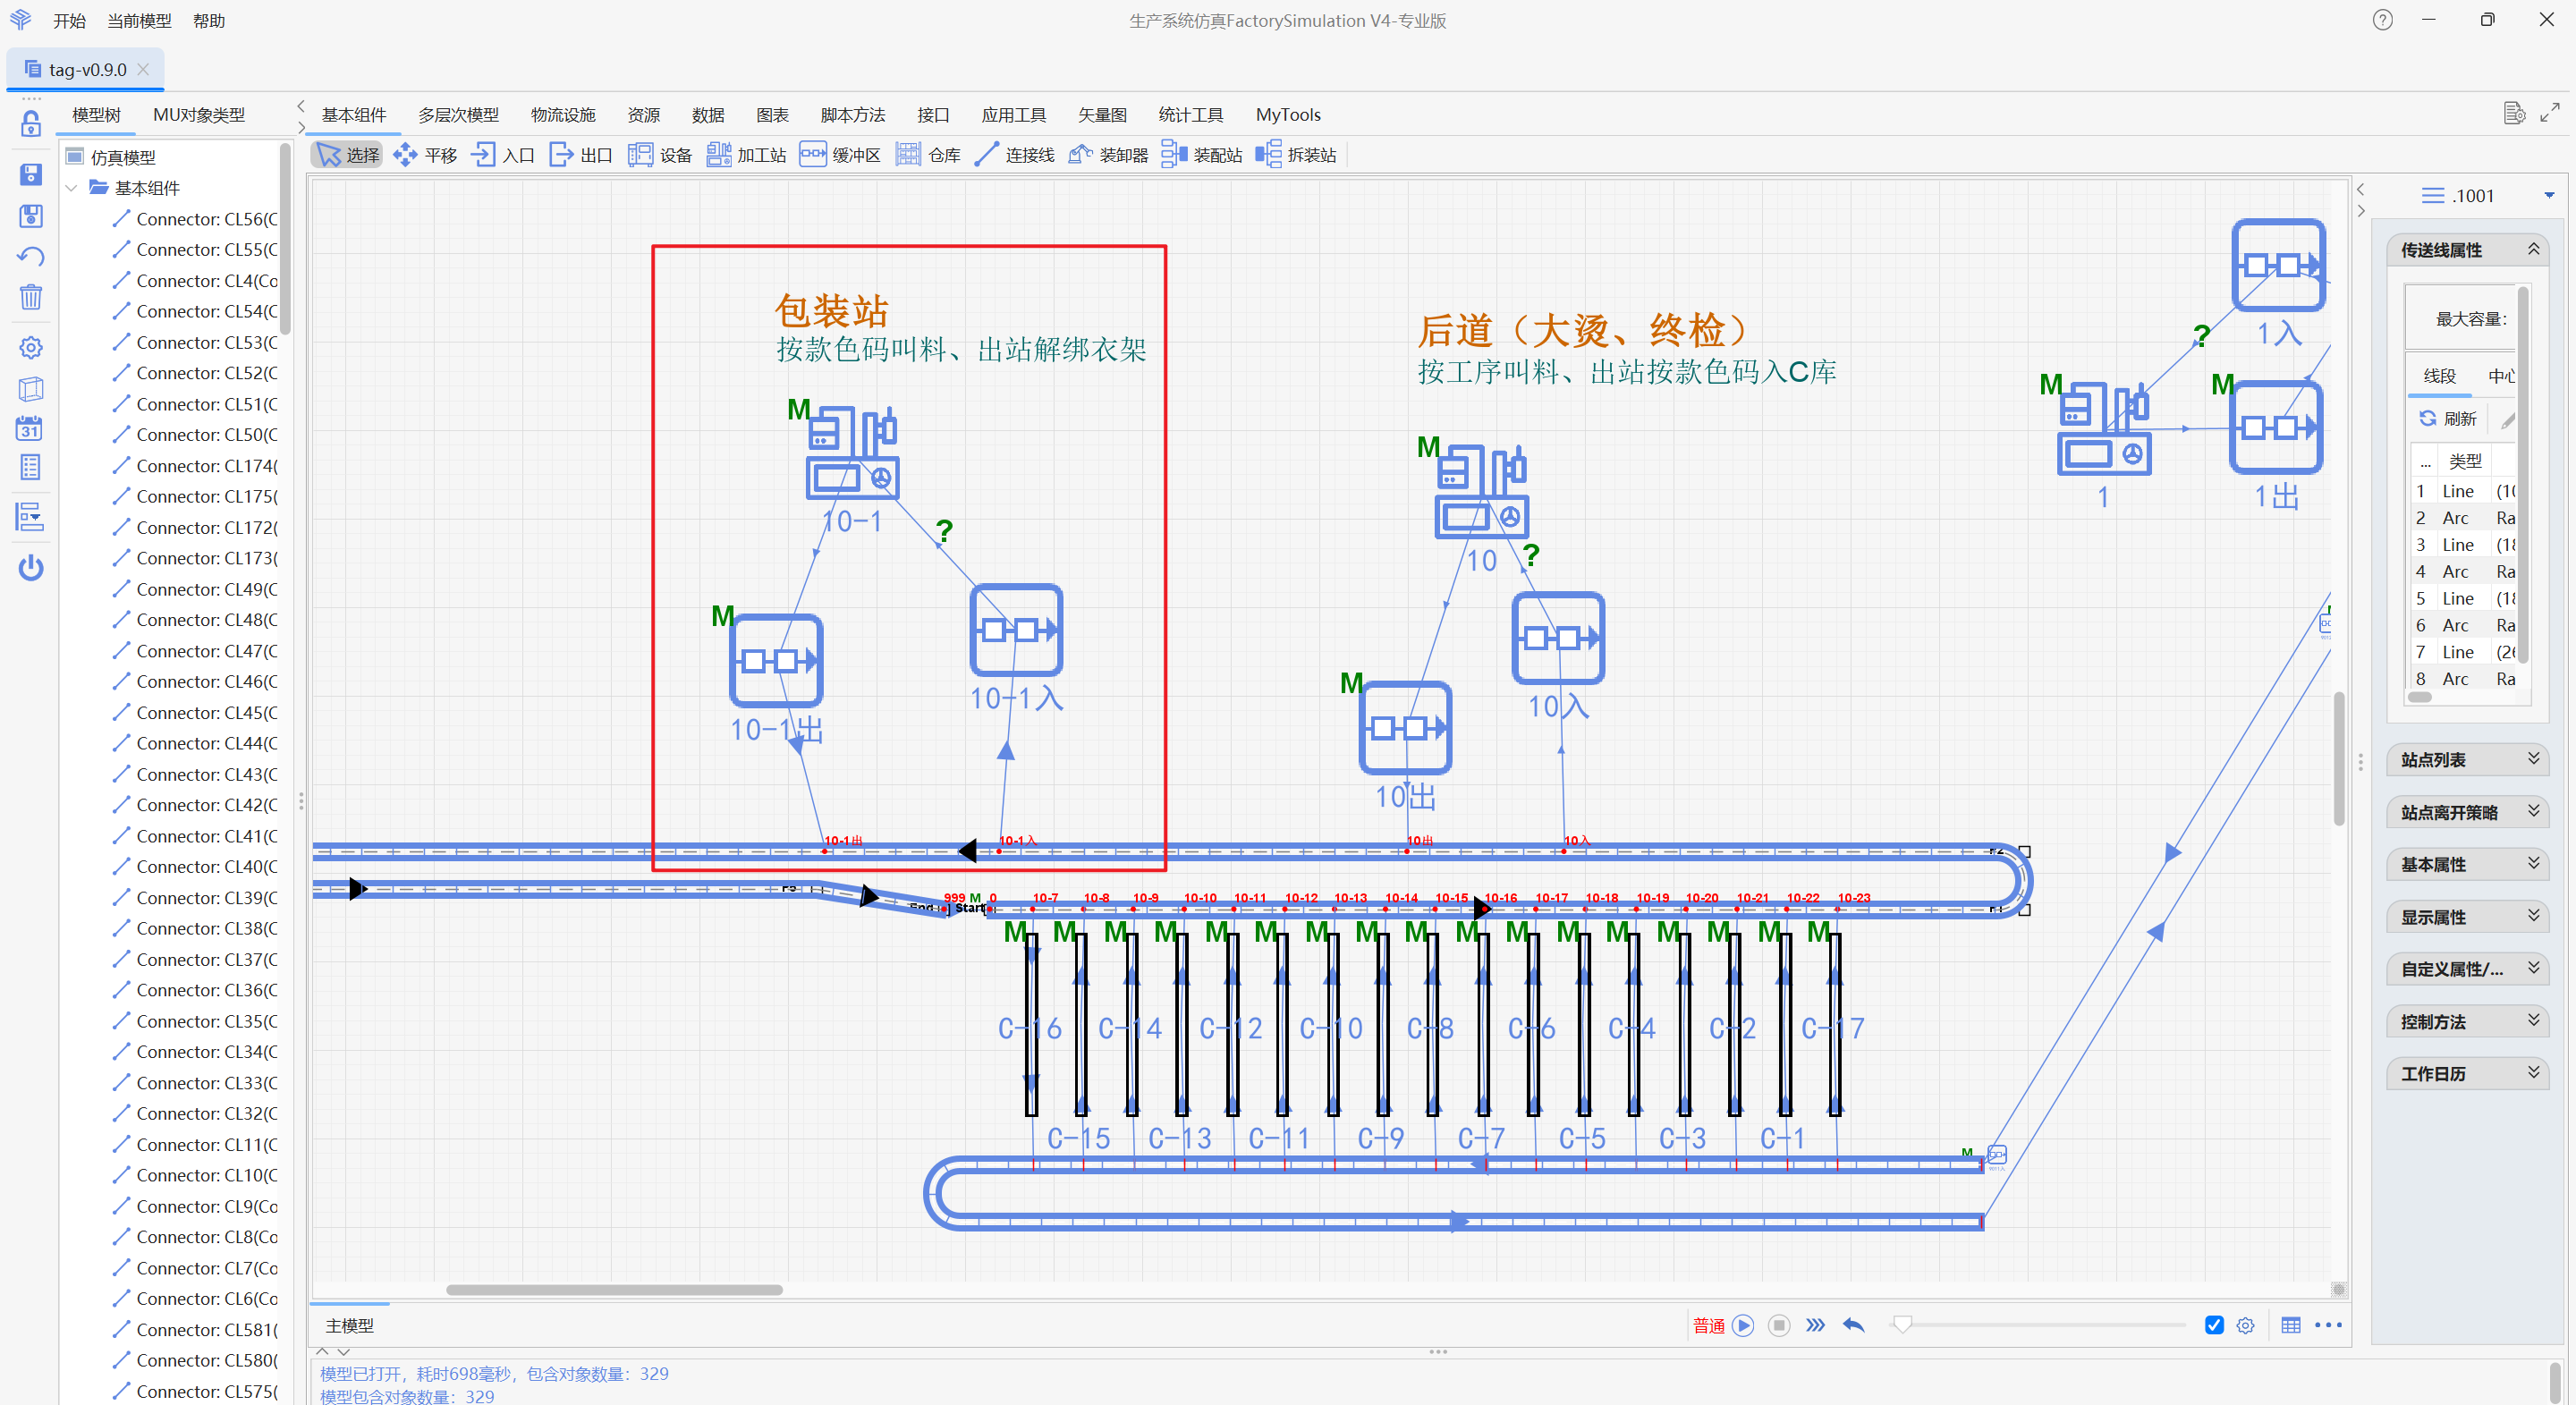
\includegraphics[width=0.8\textwidth]{pics/jack/packing-station.png}
			\caption{模型增加包装站}\label{fig:packing-station}
		\end{figure}
		\item \it{添加包装站}：复制后道模型并重命名（入站缓冲区“10-1入”、加工站“10-1”、出站缓冲区“10-1出”）,添加入站、出站缓冲区。
	\end{itemize}
	\item \bf{测试桩修改}
	\begin{itemize}
		\item \it{工序增加是否空衣架叫料属性}：不再以是否是首道工序为空衣架叫料依据。包装排产单就是从成衣仓叫料。
		\item \it{工序增加解绑衣架属性}：不再以是否有下序判断是否解绑衣架。解绑衣架为 true 时，出站衣架回空衣架存储杆，否则入指定仓。
		\item \it{增加包装排产单}：有上述两个属性，可单独进行包装排产。
		\item \it{对应的基础数据修改}：1001主轨增加两个节点：10-1入、10-1出。
		\item \it{末道工序不解绑的处理}：按 “款”、“色”、“码” 属性入库。
		\begin{enumerate}[label=\alph*)]
			\item \it{添加neum类}: 定义出入库出入仓的 props 属性
			\item \it{衣架属性增加}：“款”、“色”、“码” 等属性
			\item \it{首工序随机给属性赋值}：两款、三色、四码
			\item \it{末道工序不解绑入库}：入库的 props 只提供key，value为“”，根据衣架的属性值，找符号混存要求的库位
		\end{enumerate}
		\item \it{增加包装排产单}：按C库中衣架的属性值进行统计，按指定属性出库
		\begin{enumerate}[label=\alph*)]
			\item \it{前端多级联动查询统计C库衣架的属性}：款、色、码、PO、排产单、工序、制单、款号、流水线号，先选的优先级高，可任意组合
			\item \it{组合完毕后，可知最大数量}：可指定包装排产数量
			\item \it{提交包装排产单}：状态机变量增加props属性，以便在出库接口调用时使用
		\end{enumerate}
	\end{itemize}
\end{enumerate}
